\chapter{Anhang}

\section{Ein kurzer Überblick - die Funktionseinheiten des Arduino Uno}
\label{sec:ueberblick}
Im Folgenden wird ein vertiefter Überblick über die wichtigsten Komponenten des Arduino Uno, den sogenannten Funktionseinheiten, gegeben (vgl. Abb. \ref{abb:uno_r3}).

\begin{figure}[h]
	\centering
	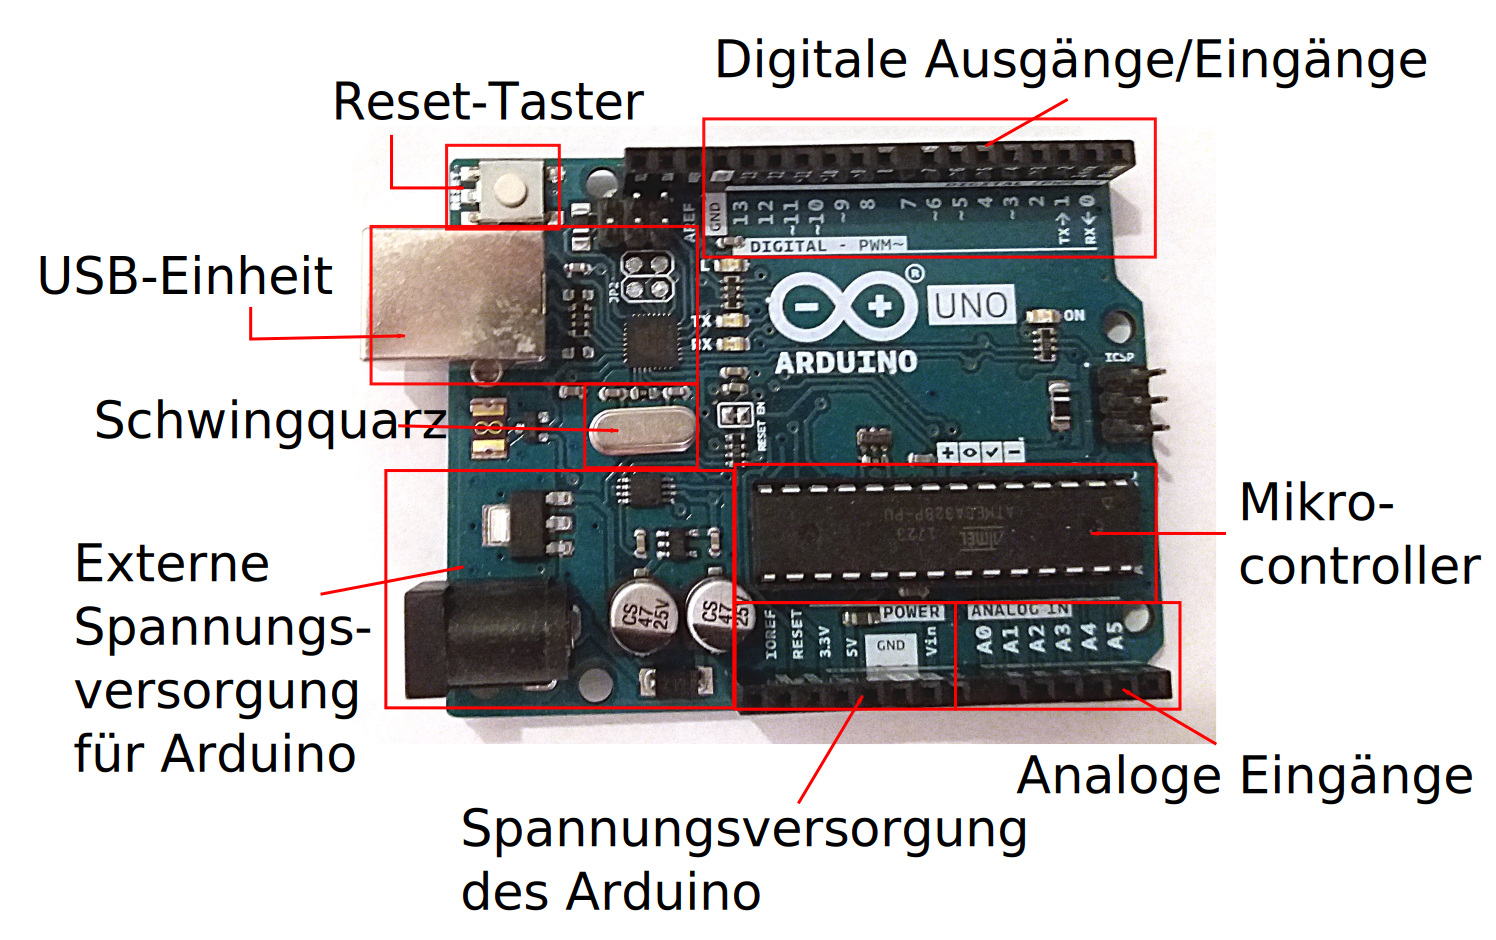
\includegraphics[width=0.8\textwidth]{pics/arduino-beschriftet.png}
	\caption{Der Arduino Uno lässt sich in wenige Funktionseinheiten aufteilen (weitere Erklärungen im Text).}
	\label{abb:uno_r3}
\end{figure}

\textbf{Mikrocontroller:} Wenn der Arduino Uno als Mikrocontroller bezeichnet wird, dann stimmt das eigentlich nicht ganz. Der eigentliche Mikrocontroller, auf dem das Programm läuft, ist das markierte schwarze Bauteil, bei dem es sich um einen Atmega328\index{Atmega328} handelt. Die Arbeit von Massimo Banzi und David Cuartielles unter anderem bestand darin, die restlichen Bauteile, die zur Verwendung des Mikrocontrollers benötigt werden, zusammen mit dem Atmega328 auf einem Board zu befestigen. Dadurch wurde die Handhabung wesentlich vereinfacht! Auf dem Mikrocontroller befindet sich ein sogenannter Bootloader, der das Programm vom Computer in den Speicher des Mikrocontrollers lädt.

\textbf{Schwingquarz:} Der Atmega328P arbeitet mit einer Taktfrequenz von 16 MHz, die von dem Schwingquarz vorgegeben wird. Das heißt, es werden pro Sekunde 16\,000\,000 \enquote{Arbeitsschritte} vollzogen! Natürlich sind moderne Computer noch viel schneller, aber für unsere Zwecke reicht das völlig aus.

\textbf{Stromversorgungseinheit:} Natürlich benötigt ein Mikrocontroller Strom oder besser gesagt eine gewisse Spannung, um funktionieren zu können. An der schwarzen Buchse können Gleichspannungsquellen zwischen $\SI{7}{\volt}$ und $\SI{12}{\volt}$ angeschlossen werden, um den Mikrocontroller mit Energie zu versorgen. Die anderen Bauteile regeln diese Spannung dann auf die $\SI{5}{\volt}$ herunter, die der Mikrocontroller zum Arbeiten benötigt.

\textbf{USB-Einheit:} An der silbernen Buchse kann das USB-Kabel angeschlossen und der Arduino Uno somit mit dem Computer verbunden werden. Dies ermöglicht die Übertragung eines Programms auf den Arduino Uno. Außerdem lassen sich dadurch weitere Daten, z.B. von Sensoren am Arduino Uno, mit dem Computer austauschen. Der USB-Anschluss dient außerdem bereits als Spannungsversorgung. Solange der Arduino Uno am Computer angeschlossen ist, braucht man in der Regel keine Batterie als zusätzliche Spannungsversorgung. Eine Ausnahme sind Motoren, denn der USB-Anschluss stellt \emph{maximal 500\,mA} bereit und Motoren benötigen häufig mehr. Glücklicherweise ist die USB-Buchse gegen Überstrom geschützt und schaltet sich bei einem Kurzschluss automatisch ab.

\textbf{Digitale Eingänge und Ausgänge:} Die digitalen Pins lassen sich entweder als Ausgänge oder als Eingänge benutzen. Wenn sie als Ausgang festgelegt werden, dann kann dort eine Spannung von 0\,V oder 5\,V angelegt werden. Wenn sie als Eingang festgelegt werden, können dort Spannungen von 0\,V oder 5\,V eingelesen werden. Einige Pins sind mit einer Tilde ($\sim$) gekennzeichnet, was bedeutet, dass sie über eine Pulsweitenmodulation verfügen. Der GND-Pin stellt den negativen Pol dar (auch Erdung oder GrouND genannt).

Hinweise: 
\begin{itemize}
	\item Die \textbf{maximale Stromstärke}, die die Digitalpins vertragen, ist \textbf{40\,mA}. Empfohlen sind eher 20\,mA.\footnote{Weitere Infos finden sich unter \url{https://playground.arduino.cc/Main/ArduinoPinCurrentLimitations}.}
	\item Pin 0 und Pin 1 sind bei angeschlossenem USB-Kabel für die Kommunikation mit dem Computer belegt und können daher nicht benutzt werden, wenn der Arduino Uno mit dem Computer kommunizieren soll!
\end{itemize}

\textbf{Spannungsversorgung:} Hiermit ist die Spannungsversorgung für die Bauteile gemeint, die man an den Arduino anschließt. Diese Pins lassen sich nicht über das Programm an- und ausstellen, sondern liefern permanent eine gewisse Spannung ($\SI{5}{\volt}$ bzw. $\SI{3,3}{\volt}$), die mit den GND-Pins geerdet wird. Der RESET-Pin wird in diesem Skript nicht genutzt, weil man den Reset über die Reset-Taste durchführen kann (siehe unten). Mit VIN kann eine Referenzspannung (Vergleichsspannung) eingelesen werden. Der IOREF-Pin legt fest, ob der Mikrocontroller mit $\SI{5}{\volt}$ oder mit $\SI{3,3}{\volt}$ operiert. Standardmäßig sind $\SI{5}{\volt}$ eingestellt.

Hinweis: Die \textbf{maximale Stromstärke}, die der 5V-Pin sowie die GND-Pins vertragen, ist \textbf{$\SI{200}{\milli\ampere}$}.

\textbf{Analoge Eingänge:} An analogen Eingängen kann eine Spannung eingelesen werden. Dabei sind nicht nur zwei Werte möglich (wie bei den digitalen Eingängen), sondern auch viele Werte zwischen $\SI{0}{\volt}$ und $\SI{5}{\volt}$.

\textbf{Reset-Taste:} Mit der Reset-Taste lässt sich der Arduino neu starten. Dabei wird das Programm, das auf den Arduino geladen wurde, nicht gelöscht, sondern lediglich neu gestartet.

%\section{Das Elegoo Starter-Kit}
%\label{sec:starter_kit_elegoo}
%
%Bei Erstellung dieses Skripts wurde ein günstiges Starter-Kit von Elegoo genutzt, das alle grundlegenden elektronischen Bauteile enthält. Der darin enthaltene Mikrocontroller \enquote{Elegoo Uno R3} wurde nach dem frei verfügbaren Aufbau des Arduino nachgebaut, darf aber nicht Arduino genannt werden, weil die Namensrechte bei der Firma tinker.it liegen. Der Nachsatz \emph{Uno R3} spielt auf die aktuelle Version des am weitesten verbreiteten Arduino Uno R3 an. Es folgt eine Übersicht aller Bauteile des Starter-Kits:
%\begin{multicols}{2}
%	\begin{itemize}
%		\item 1 x UNO R3 Mikrocontroller,
%		\item 1 x LCD1602 Display (mit fertig verlötetem Pin Header),\index{LC-Display}
%		\item 1 x DHT11 Modul (Temperatur- und Feuchtigkeitssensor),
%		\item 1 x Joystick-Modul,\index{Joystick}
%		\item 1 x 5V Relais,\index{Relais}
%		\item 1 x MB-102 Breadboard (Steckbrett),
%		\item 1 x Servomechanismus(SG90),\index{Servo}
%		\item 1 x Schrittmotor,\index{Schrittmotor}
%		\item 1 x ULN2003 Schrittmotor-Treibermodul,
%		\item 1 x Prototyp-Erweiterungsplatine,
%		\item 1 x Power Supply Module,
%		\item 1 x Ultraschall-Sensor-Modul,\index{Ultraschall-Sensor}
%		\item 1 x IR-Empfängermodul,
%		\item 1 x IR-Fernbedienung,
%		\item 1 x 3V Gleichstrommotor,
%		\item 1 x USB Kabel,
%		\item 1 x 65 M-M Kabel,
%		\item 1 x 10 Female-to-Male Kabel,
%		\item 1 x 9 V Akku mit DC,
%		\item 1 x Kugelschalter,\index{Kugelschalter}
%		\item 1 x Segmentanzeige,\index{Segmentanzeige}
%		\item 1 x 4x7-Segment-Anzeige,\index{Segmentanzeige!4x7}
%		\item 1 x IC 74HC595 (Schieberegister),\index{Schieberegister}
%		\item 1 x Aktiver Summer,\index{Summer!aktiv}
%		\item 1 x Passiver Summer,\index{Summer!passiv}
%		\item 1 x Potentiometer,\index{Potentiometer}
%		\item 1 x Thermistor,\index{Thermistor}\index{NTC}
%		\item 1 x Diode Rectifier (1N4007),
%		\item 2 x NPN Transistor (pn2222),\index{Transistor}
%		\item 2 x LDR (Fotowiderstand),\index{Fotowiderstand}\index{LDR}
%		\item 1 x RGB LED,\index{LED!RGB}
%		\item 5 x weiße LED,
%		\item 5 x gelbe LED,
%		\item 5 x Blaue LED,
%		\item 5 x grüne LED,
%		\item 5 x rote LED,
%		\item 5 x Druckschalter,\index{Taster}
%		\item 10 x 10 Ohm-Widerstand,\index{Widerstand}
%		\item 10 x 100 Ohm-Widerstand,
%		\item 30 x 220 Ohm-Widerstand,
%		\item 10 x 330 Ohm-Widerstand,
%		\item 10 x 1k Ohm-Widerstand,
%		\item 10 x 2k Ohm-Widerstand,
%		\item 10 x 5k1 Ohm-Widerstand,
%		\item 10 x 10k Ohm-Widerstand,
%		\item 10 x 100k Ohm-Widerstand,
%		\item 10 x 1m Ohm-Widerstand,
%		\item 1 x Fan,
%		\item 1 x L293D (4 Kanal Treiber mit Diode).
%	\end{itemize}
%\end{multicols}
%
%Zusätzlich wurden Bewegungsmelder angeschafft.

\section{Installation der integrierten Entwicklungsumgebung (IDE) für den Arduino}
\label{sec:install_ide}

Üblicherweise wird der Arduino mit der integrierten Entwicklungsumgebung (IDE - engl. \emph{integrated development environment}), die ebenfalls Arduino heißt, programmiert. Diese verfügt über einen Texteditor, in dem das Programm geschrieben werden kann. Zusätzlich lassen sich hier einfach die Bibliotheken und weiteren Boards verwalten und einbinden. Wichtig ist zudem die Syntax-Prüfung sowie letztendlich die Kompilation des Programms. Das Programm wird in der maschinennahen Programmiersprache C++ geschrieben, für die jedoch einige vorgefertigte Befehle für den Arduino bereitgestellt werden, damit der Einstieg leichter fällt. Das Kompilieren des Programms macht aus dem Programmcode einen maschinenlesbaren Code (von Einsen und Nullen), der dann auf den Arduino übertragen wird.

Die IDE lässt sich im Internet auf der Projekthomepage für jedes Betriebssystem herunterladen:

\url{https://www.arduino.cc/en/Main/Software}.

Auf derselben Seite gibt es zudem ausführliche Anleitungen zur Installation (englisch):

\url{https://www.arduino.cc/en/Guide/HomePage}.

Eine ebenfalls ausführliche und deutschsprachige Installationsanleitung wird auf der CD des Starter Kits mitgeliefert.

\section{Mit der Arduino IDE ein Programm auf den Arduino Uno übertragen}
\label{sec:program_ide}

Nach Installation der Entwicklungsumgebung kann das erste, noch leere Programm auf den Arduino Uno übertragen werden, um zu testen, ob und wie das Ganze funktioniert. Dazu wird der Arduino Uno mit dem USB-Kabel an den PC angeschlossen und die Arduino-Entwicklungsumgebung geöffnet. Wenn der Arduino Uno zum ersten Mal an den PC angeschlossen wird, muss evtl. kurz gewartet werden, damit die Treiber für die Kommunikation von PC und Arduino Uno installiert werden. Das passiert aber vollautomatisch.

\begin{figure}[H]
	\centering
	\includegraphics[width=0.8\textwidth]{pics/ide-ueberblick.png}
	\caption{Ein Überblick über die Arduino-Entwicklungsumgebung.}
	\label{abb:ide}
\end{figure}

In der Mitte des Fensters der Entwicklungsumgebung wird das Programm geschrieben. Innerhalb der geschweiften Klammern von \texttt{void setup()} werden Anweisungen geschrieben, die ganz am Anfang genau einmal ausgeführt werden. Im Setup befindet sich bereits ein Kommentar, der sich daran erkennen lässt, dass er eine graue Farbe hat. Kommentare werden im Programm dadurch gekennzeichnet, dass am Anfang zwei Schrägstriche stehen. Sie sind nützlich, um in komplizierteren Programmen auch später noch den Überblick zu behalten und um anderen, die das Programm nutzen wollen, die Möglichkeit zu geben, es zu verstehen.

Innerhalb der geschweiften Klammern von \texttt{void loop()} stehen Anweisungen, die immer wieder wiederholt werden. Die Anweisungen werden der Reihe nach abgearbeitet und nach dem letzten Befehl beginnt der Arduino Uno wieder mit dem ersten Befehl innerhalb des Loops, der auf Deutsch entsprechend Schleife heißt. In dieser unendlichen Schleife wird der Hauptteil des Programms stehen.

\medskip
\ausrufezeichen Für den Einstieg ist es am einfachsten, den Quelltext von Nepo zu kopieren, nachzuvollziehen und anzupassen. Um den Quelltext von Nepo in der Arduino IDE nutzen zu können muss lediglich die Zeile \texttt{\#include <NEPODefs.h>} entfernt werden.

\medskip

Die wesentlichen anderen Bestandteile der Entwicklungsumgebung werden im Folgenden erklärt.

1. \emph{Sketch überprüfen:} Mit dem Haken kann überprüft werden, ob das Programm, das in der Arduino-Welt auch Sketch genannt wird, richtig geschrieben ist. Damit ist natürlich nicht der Inhalt gemeint, denn die Entwicklungsumgebung weiß natürlich nicht, was das Programm bewirken soll. Es wird nur überprüft, ob die \enquote{Grammatik} (Fachwort: die Syntax) des Programms richtig ist. So wie in einem Satz die Wörter in einer bestimmten Reihenfolge stehen und ggf. mit Kommata getrennt werden müssen, müssen in einer Programmiersprache Befehle korrekt geschrieben, geöffnete Klammern wieder geschlossen und das Ende von Befehlen mit einem Semikolon deutlich gemacht werden. Genau das wird mit dem Haken überprüft.

2. \emph{Sketch überprüfen und hochladen:} Mit dem Pfeil wird der Sketch nicht nur überprüft, sondern auch auf den Arduino Uno hochgeladen.

3. \emph{Serieller Monitor:} Mit dem seriellen Monitor kann man Daten vom Arduino Uno abfragen und am Computer anzeigen lassen. Man kann auch umgekehrt Daten am Computer eingeben und vom Arduino auslesen lassen. Wenn man ihn entsprechend programmiert, kann man dem Arduino auf diese Weise auch während der Durchführung des Programms noch Befehle geben.

4. \emph{Informationen zum Überprüfen und Hochladen:} Beim Überprüfen und Hochladen zeigt die Entwicklungsumgebung in dem schwarzen Bereich Informationen zum Fortschritt und ggf. zu Fehlern an.

5. \emph{Statuszeile:} In der Statuszeile sieht man, welcher Arduino-Typ ausgewählt wurde (in diesem Skript ist das immer der Arduino Uno) und an welchem USB-Port er sich befindet. Dargestellt ist der Pfad unter Linux - unter Windows werden die Ports mit COM1, COM2, ... bezeichnet.

\begin{zsfg}{Fehlerursachen}
	
	Eine häufige Fehlerursache, die das Hochladen verhindert, ist, dass kein oder ein falscher USB-Port ausgewählt wurde. Der USB-Port muss unter Werkzeuge -> Port ausgewählt werden. In der Regel ist dort nur der eine Port auswählbar, an dem sich der Arduino Uno befindet. Falls kein Port auswählbar ist, fehlt der Treiber für die Kommunikation von Arduino und Computer. Er muss dann manuell nachinstalliert werden.
\end{zsfg}